%this file is the first report
%a % comment anything after % until the end of the line

%minimum references to begin our article
\documentclass[12pt]{article}
\usepackage[frenchb]{babel}
\usepackage[utf8]{inputenc}
\usepackage[T1]{fontenc}
\usepackage{graphicx}
\usepackage{fancyhdr}
\usepackage{hyperref}
\usepackage{float}
\usepackage{amsmath}
\usepackage[margin=1in]{geometry}
\usepackage{indentfirst}
\usepackage[section]{placeins}


\pagestyle{fancy}
%\cfoot{Insattack : Projet de POO}
% the last extension makes it possible to add images

%presentation of the document
\title{Insattack : Projet de POO\smallbreak Rapport de conception}
\author{Baptiste \textsc{Bignon}, Gabriel \textsc{Prevosto}}
\date{12/11/2014}
\setlength\parindent{15pt}
\begin{document}

\maketitle
\vfill %tous les vfill prennent la même place

\begin{figure}[!h]
\centering

\includegraphics[width=\textwidth]{Parties/Images/Logo}
\label{fig:logo}
\end{figure}

\vfill
\vfill
\newpage

%to add a table of contents
\tableofcontents
\renewcommand{\contentsname}{Sommaire}
\newpage


\section{Introduction}			\label{sec:introduction}			Notre projet a pour but la création du jeu \emph{Insattack}, dérivé de Small World qui au lieu d'appartenir à un univers fantastique sera une réprésentation de l'INSA. Pour cela nous avons étudié le fonctionnement du jeu et réalisé la conception du modèle. Celui-ci est prévu pour être facilement adaptable, afin de pouvoir ajouter ou modifier des régles, car celles-ci ne sont pas encore fixées pour un soucis d'équilibrage.

L'interface graphique n'a pas encore été étudiée, mais l'utilisation du modèle MVC pour l'implémentation du jeu permettra de l'intégrer faiclement.
\newpage

\section{Le jeu}				\label{sec:jeu}
\subsection{Les règles}			\label{sec:regles}				\subsubsection{Principe du jeu}
INSAttack est un jeu à deux joueurs au tour par tour, chaque joueur choisit son département parmi : INFO, EII, SRC, SGM, GMA, GC. En fonction de son choix ses unités disposeront de différentes capacités (voir partie\ref{sec:departements}). Au début du jeu, les unités de chaque joueur sont rassemblés sur sa case de départ. Afin de gagner la partie un joueur doit éliminer toutes les unités adverses ou avoir un maximum de points à la fin du nombre de tours imparti. Pour cela chaque case qu'il posséde une lui rapporte 2 point. Certains départements peuvent aussi gagner des points grâce à leurs capacités, ou gagner plus ou moins de points selon les types de cases contrôlés.

\subsubsection{Les déplacements}
Pour déplacer une unité, il faut faire un clic gauche sur la case la contenant, puis sur l'unité voulue dans la liste qui s'affichera sur la gauche. Une fois cela fait vous pouvez la déplacer sur une case en faisant un clic droit dessus. L'unité se déplacera si le mouvement est possible, c'est à dire si elle posséde suffisament de points de déplacement et si la case est adjacente.

\subsubsection{Les combats}
Vous pouvez bien sûr attaquer les unités adverses simplement en déplaçant l'une de vos unités sur la case où se trouve votre cible. Le combat sera alors déclenché, un nombre de tour sera choisi aléatoirement, durant chacun d'entre eux les chances de gagner de l'attaquant seront calculées en fonction de son attaque et de la défense de son adversaire. L'unité qui perd un tour de combat perd 1 point de vie. Le combat se termine si l'une des unités meurt ou que tous les tours ont été réalisés. Si l'unité ciblée est morte l'attaquant se déplace sur la case qu'elle occupait. Quelle soit réussie ou non, une attaque consomme autant de points de déplacement qu'un mouvement vers cette case.
\subsection{Les peuples}			\label{peuples}				Au lieu de choisir des peuples fantastiques comme les orcs ou les elfes, nous avons décidé d'utiliser les départements de l'INSA : INFO, SRC, EII, SGM, GMA et GC. Nous n'avons pas encore fixé les bonus dont bénificiera chaque peuple mais nous prévoyons d'ajouter différents effets à ceux existant déjà. Par exemple des bonus d'attaque ou de défense sur certaines cases, ou divers moyens de gagner des points supplémentaires.
\subsection{Les terrains}			\label{terrains}				Nous remplacerons les terrains proposés initialement par différentes salles de l'INSA. Ainsi, les terrains basiques seront les salles de TD, les amphithéâtres ou encore les salles informatiques. Nous avons aussi comme projet l'ajout de cases spéciales uniques et disposant d'effets particuliers non liés au peuple de l'unité se trouvant dessus. Par exemple, toute unité présente sur la case du self à la fin d'un tour pourra subir aléatoirement un gain ou une perte de PV.
Actuellement, tous les terrains ne sont pas fixés. Comme nous créons plus de peuples que le jeu de base, nous ajouterons peut-être également d'autres types de cases afin d'équilibrer le jeu et de faire varier les bonus des peuples.
\newpage

\section{Architecture}			\label{sec:archi}
\subsection{Architecture principale}	\label{sec:architecturePrincipale}		Afin de réaliser un project structuré et plus facilement adaptable, nous avons décidé de le séparer en différents modules. Nous implémenterons le jeu en suivant le patron modéle-vue-contrôleur (\emph{MVC}) qui consiste à séparer totalement les données de l'interface graphique et de la gestion des entrées. On peut ainsi par exemple remplacer une vue par une autre sans difficulté. Par ailleurs si le project principal sera développé en C\# et utilisera WPF pour l'interface, une librairie C++ sera créée pour gérer les règles du jeu.
\subsection{Création d'une partie}	\label{sec:creationPartie}			Afin de comprendre comment se déroule la création d'une partie, nous avons réalisé deux diagrammes.

Le premier, un diagramme de cas d'utilisation, nous permet d'illustrer les actions que le joueur est autorisé à faire lorsqu'il lance le jeu et choisit la partie à laquelle il veut jouer.
\begin{figure}[!h]
\centering
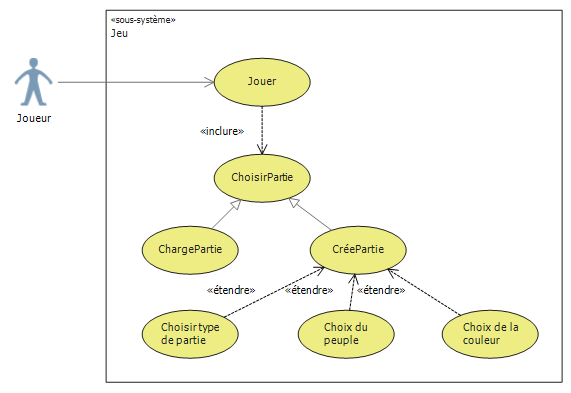
\includegraphics[width=\textwidth]{Parties/Images/cdu_CreationPartie.png}
\caption{Diagramme de cas d'utilisation : création d'une partie}
\label{fig:cdu_CreationPartie}
\end{figure}

\newpage
Ensuite nous avons créé un diagramme de séquence afin de déterminer la hiérarchie de création des différents éléments du jeu.
\begin{figure}[!h]
\centering
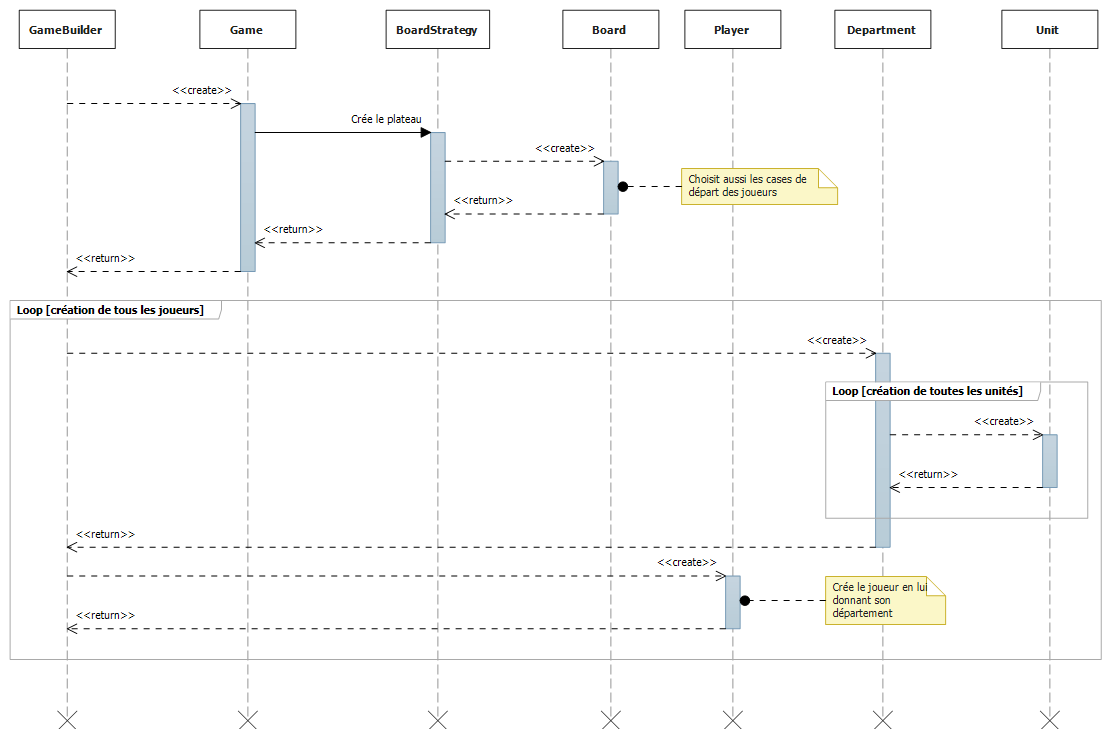
\includegraphics[width=\textwidth]{Parties/Images/seq_CreationPartie.png}
\caption{Diagramme de séquence : création d'une partie}
\label{fig:seq_CreationPartie}
\end{figure}

\newpage
\subsection{Déroulement d'une partie}	\label{sec:deroulementPartie}		Afin de comprendre comment se déroule  une partie, nous avons réalisé un diagramme de cas d'utilisation. Ce diagramme nous permet d'indiquer les actions que le joueur est autorisé à faire dans le fonctionnement normal du jeu.
\begin{figure}[!h]
\centering
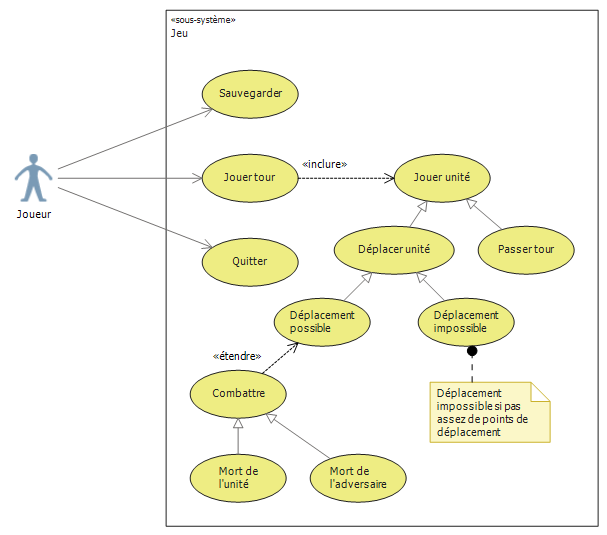
\includegraphics[width=\textwidth]{Parties/Images/cdu_TourDeJeu.png}
\caption{Diagramme de cas d'utilisation : tour de jeu}
\label{fig:cdu_TourDeJeu}
\end{figure}

\newpage
\subsection{Cycle de vie des unités}	\label{sec:cycleVieUnites}			Nous avons aussi modélisé le cycle de vie des unités à l'aide de deux diagrammes.

Le premier, un diagramme d'états-transitions nous permet de visualiser les différents cas posisbles lors du déplacement d'une unité et les différentes possibilités qui en découlent.
\begin{figure}[!h]
\centering
\includegraphics[width=\textwidth]{Parties/Images/CycleVieUnité.png}
\caption{Diagramme d'états-transitions : cycle de vie d'une unité}
\label{fig:CycleVieUnité}
\end{figure}

\newpage
Ensuite nous avons créé un diagramme de séquence afin d'illustrer les traitements effectués par le jeu lorsque le joueur déplace une unité, c'est à dire la vérification de la validité du mouvement, et s'il est réalisable son éxécution ainsi que la résolution du combat si une unité adversaire est présente sur la case de destination.
\begin{figure}[!h]
\centering
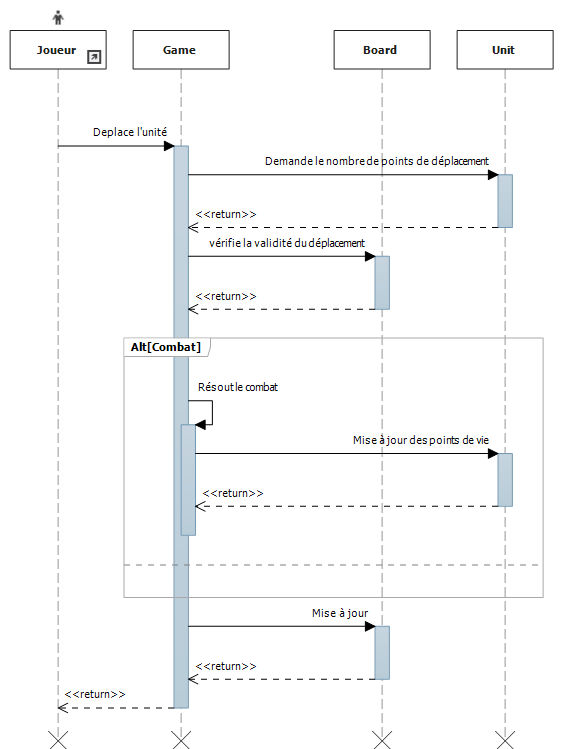
\includegraphics[width=\textwidth]{Parties/Images/seq_DeplacementUnite.png}
\caption{Diagramme de séquence : déplacement d'une unité}
\label{fig:seq_DeplacementUnite}
\end{figure}

\newpage

\section{Implémentation}			\label{sec:implementation}
\subsection{Diagramme de classes}	\label{sec:diagrammeClasses}		\input{"Parties/DiagrammeClasses.tex"}
\subsection{Patrons de Conception}	\label{sec:patronsConception}		\input{"Parties/PatronsConception.tex"}
\newpage

\section{Conclusion} 			\label{sec:conclusion}			La conception du modèle pour le jeu \emph{Insattack} est finie, son implémentation peut donc commencer.
L'interface utilisateur n'a pas encore été pensée ; cependant, le modèle n'y fait pas référence et peut donc être développé avant.
Par la suite, l'interface graphique utilisera le modèle pour gérer la partie.

Les règles du jeu ont été légèrement modifiées afin de correspondre avec l'environnement de l'INSA ; il sera donc peut-être nécessaire de les modifier à nouveau dans un souci d'équilibrage.
Cependant, ces modifications seront simples à effectuer grâce à l'utilisation des patrons de  conception décrits dans la partie \ref{sec:patronsConception}.


\end{document}
